%%
%% This is file `sample-sigconf.tex',
%% generated with the docstrip utility.
%%
%% The original source files were:
%%
%% samples.dtx  (with options: `sigconf')
%% 
%% IMPORTANT NOTICE:
%% 
%% For the copyright see the source file.
%% 
%% Any modified versions of this file must be renamed
%% with new filenames distinct from sample-sigconf.tex.
%% 
%% For distribution of the original source see the terms
%% for copying and modification in the file samples.dtx.
%% 
%% This generated file may be distributed as long as the
%% original source files, as listed above, are part of the
%% same distribution. (The sources need not necessarily be
%% in the same archive or directory.)
%%
%%
%% Commands for TeXCount
%TC:macro \cite [option:text,text]
%TC:macro \citep [option:text,text]
%TC:macro \citet [option:text,text]
%TC:envir table 0 1
%TC:envir table* 0 1
%TC:envir tabular [ignore] word
%TC:envir displaymath 0 word
%TC:envir math 0 word
%TC:envir comment 0 0
%%
%%
%% The first command in your LaTeX source must be the \documentclass command.
\documentclass[sigconf,authorversion,noacm]{acmart}
\settopmatter{printacmref=false}

%%
%% \BibTeX command to typeset BibTeX logo in the docs
\AtBeginDocument{%
  \providecommand\BibTeX{{%
    Bib\TeX}}}

\setcopyright{none}
\acmConference[CS536 Fall 2022]{CS536 Fall 2022}{Aug 24--Dec 15 2022}{West
Lafayette, IN, USA}

%% Rights management information.  This information is sent to you
%% when you complete the rights form.  These commands have SAMPLE

%%
%% end of the preamble, start of the body of the document source.
\begin{document}

%%
%% The "title" command has an optional parameter,
%% allowing the author to define a "short title" to be used in page headers.
\title{Improving cache allocation for networking applications using fine-grained
cache partitioning and unikernels}

%%
%% The "author" command and its associated commands are used to define
%% the authors and their affiliations.
%% Of note is the shared affiliation of the first two authors, and the
%% "authornote" and "authornotemark" commands
%% used to denote shared contribution to the research.
\author{Jiangqiong Liu}
\email{liu3328@purdue.edu}
\affiliation{
    \institution{Purdue University}
    \country{United States}}

\author{Joshua Reprogle}
\email{jreprogl@purdue.edu}
\affiliation{
    \institution{Purdue University}
    \country{United States}}

\author{Vedaant Rajoo}
\email{vrajoo@purdue.edu}
\affiliation{
    \institution{Purdue University}
    \country{United States}}

\author{Sowmya Jayaram Iyer}
\email{jayarami@purdue.edu}
\affiliation{
    \institution{Purdue University}
    \country{United States}}

\author{Keerthana Ashokkumar}
\email{kashokku@purdue.edu}
\affiliation{
    \institution{Purdue University}
    \country{United States}}

\author{Anmol Sahoo}
\affiliation{
    \institution{Purdue University}
    \country{United States}}
\email{sahoo9@purdue.edu}

%%
%% By default, the full list of authors will be used in the page
%% headers. Often, this list is too long, and will overlap
%% other information printed in the page headers. This command allows
%% the author to define a more concise list
%% of authors' names for this purpose.
\renewcommand{\shortauthors}{Liu et al.}

%%
%% The abstract is a short summary of the work to be presented in the
%% article.
\begin{abstract}
    We present a solution for improving the performance of networking
    applications. The performance of network IO is bound by the delay of
    accessing main memory and thus processors implement Direct Cache Access
    (DCA) technology such as Intel DDIO to bypass the main memory and improve
    performance. But, cache contention between different parts of an application
    hurts the performance of DDIO and thus we propose a solution that minimizes
    such interference. We rely on two crucial insights - intra-application cache
    partitioning to isolate networking and non-networking parts of the code and
    deploying unikernels to remove interference from the operating system. We
    present an implementation of this solution using the Intel Resource Director
    Technology (RDT) for cache partitioning and the Unikraft unikernel library.
    Finally, we present an evaluation strategy using hardware counter events and
    report our results over a set of benchmarks.
\end{abstract}

\maketitle

\section{Introduction}

As networking interfaces start breaking the 100Gbps barrier, it is being
observed that commodity processors are not able to keep up with processing
packets at the rate required to saturate these links. With the end of Moore's
law and Dennard scaling, there is an upper limit to how many instructions can be
processed in a given interval, which limits the bandwidth achievable on
commodity processors. This is further exacerbated by the fact that memory speeds
have stayed mostly constant making main memory access the critical bottleneck
to processing packets at fast rates. To deal with this problem, modern
processors often include features implementing Direct Cache Access (DCA) which
allows peripheral devices to directly read and write data from the last-level
cache of the processor. Since the peripheral can bypass the entire main memory,
this reduces the effect of the slow memory hierarchy on the packet processing
critical path and provides a pathway to better performance, at least on paper.
But the presence of DCA does not necessarily improve performance and in certain
cases may even decrease performance. Typically, since caches are small and there
is high contention for cache space, DCA may not be able to place packets
efficiently in the cache. A thorough study of the effects of DCA on networked
applications is provided in \cite{alireza_2020}. While existing solutions to
this problem rely on using coarse grained cache partitioning to isolate
different applications, they do not consider the cache contention arising from
\textit{within} an application. As we know, the computational and networking
parts of the same application may have different cache footprints which contend
for the same amount of cache space which limits the effectiveness of DCA, since
they will evict each others cache lines due to this contention. To tackle this
problem, we develop a solution based on two key insights - intra-application
cache partitioning and unikernels. We show that these two insights together are
necessary to achieve a holistic solution that reduces the effects of cache
contention arising from within different parts of the same application.
Concretely, our contributions are as follows - 

\begin{enumerate}
    \item An interface by which networking applications can demarcate regions of
        their code that perform network IO
    \item An implementation that allows executing such applications with
        fine-grained cache partitioning as a unikernel
    \item A set of benchmarks and an evaluation strategy for checking the
        performance of our solution
\end{enumerate}

While our results look promising for some benchmarks ($\sim$10$\%$ improvement
in runtime), they are not consistent across our entire testset. We identify
areas of improvement which can improve performance consistently.

\section{Background and Motivation}

Peripheral devices rely on the use of Direct Memory Access (DMA) to perform IO
operations. DMA technology implemented in processors allows peripheral devices
to directly write to system main memory through the Peripheral Component
Interface-express (PCIe) bus. The typical flow of a network interface card (NIC)
peripheral to receive a packet is to write the incoming packet in main memory
and then signal the processor via an interrupt about this event. The processor
may perform additional processing on the packet, write a new packet to main
memory and then signal the NIC to send it out. Given this setup, the latency of
accessing main memory is the main bottleneck. At 100Gbps, a processor has 6.72ns
to process small packets. But a memory access on the order of 100ns, makes
processing packets at line rate prohibitive. To address this problem processors
implement Direct Cache Access (DCA) technology. DCA is an umbrella term to refer
to technologies that can be used to improve access time of peripheral DMA data,
by placing it in the cache. For example, a simple technique allows a cache
prefetcher to prefetch parts of the peripheral memory, thus improving access in
predictable scenarios. Intel processors implement a DCA feature named DDIO
(Direct-Data IO). In this setup, a NIC can perform DMA directly from/to the
cache bypassing the main memory altogether. This prevents the delay incurred by
the processor accessing the packet from main memory. Similarly, while writing
the packet the NIC can read the packet from the cache, avoiding the latency of
the main memory. We describe this process in detail, as it highlights the role
that cache contention plays in this situation. When a NIC receives a packet, it
writes a cache line (memory address block) into the LLC via PCIe. In this case,
DDIO overwrites the cache line if it is present in the cache (PCIe write hit /
write update) or allocates a new line if not (PCIE write miss / write allocate).
Note that in the first case, DDIO may write the packet anywhere in the cache but
in the second case, it may only allocate a packet in a specific region of the
cache implying that frequent write allocations will not make effective use of
the cache. When the processor signals the NIC to send a cache line containing
the packet, the NIC will direcly read the packet from the cache using DDIO.
Similar to the previous case, if the cache line is present in the cache then it
is a hit (PCIe read hit) otherwise it reads the cache line from main memory
(PCIe read miss). With this, it becomes possible to see how DDIO may be affected
by cache contention. The first problem is called leaky DMA
\cite{tootoonchian-resq}, where incoming packets arrive faster than they can be
processed thus evicting older packets from memory. While one solution to this is
to limit the number of RX descriptors (so that the cache space used by DDIO is
bounded) it is only a temporary patch. Small number of RX descriptors increases
the packet loss, since fewer packets can be buffered now. Similarly, limiting TX
descriptors is also another proposed solution, but reducing the number of TX
descriptors leads to inefficient utilization of the PCIe bandwidth. Thus, both
of these problems are mitigated by increasing the number of RX/TX descriptors,
but this then overloads the cache and leads to reduced DDIO efficiency. This
highlights the role that cache contention plays in determining the performance
of network IO, since it leads to the eviction of RX/TX descriptors and buffers.
A significant source of such cache contention exists within an application
itself, since an application maybe performing non-trivial memory bound
computation while simultaneously performing network IO. Having motivated the
problem, we focus on solving cache-contention between different parts of the
application with the intention of improving network performance. We provide a
simple motivating example in Fig.1. As can be seen in Fig.1(a), at a certain
point in the program's call stack, the cache is occupied by the packets that
were received due to network IO. Now, the application executes some computation
which displaces these cache lines, as seen in Fig.1(b). Now any future network
IO that may need to be performed on these packets, would need to fetch them from
main memory again. This clearly illustrates the problem of different parts of
the application contending for cache memory and thus affecting networking
performance.

\begin{figure}[h]
  \centering
  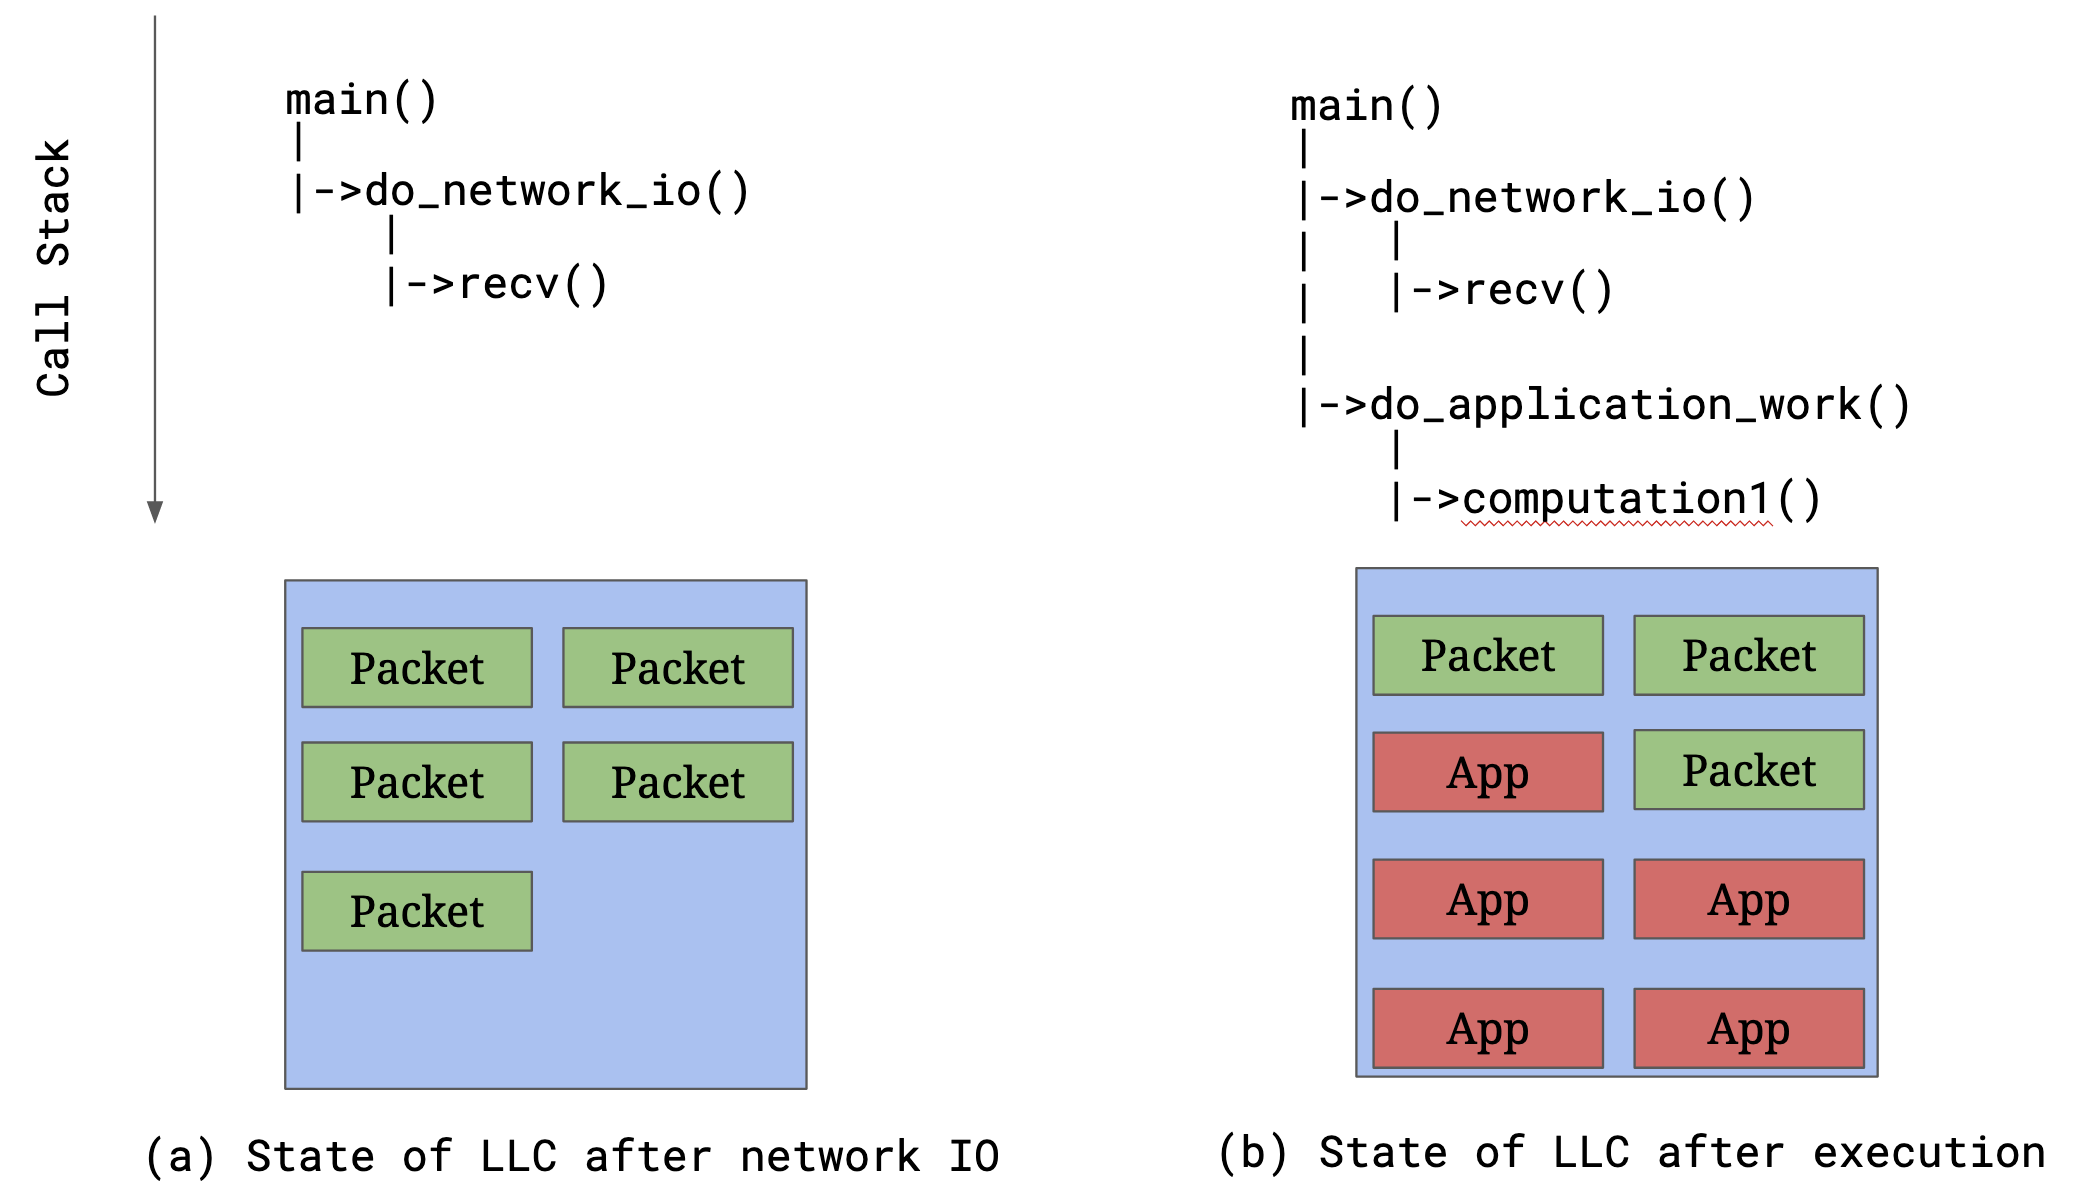
\includegraphics[width=\linewidth]{motivating_example}
    \label{fig:motivating}
    \vspace{-2em}
    \caption{Motivating Example}
    \Description{Brief representation of our contributions at different layers.
    Boxes in green represent our contribution and boxes in grey are the existing
    systems that are being reused}
\end{figure}

\section{Proposed Solution}

To mitigate the problems that we discussed in Section 2, we develop our solution
based on two key insights - (1) intra-application cache partitioning and (2)
using unikernels to remove OS contention. Intra-application cache partitioning
refers to performing fine-grained partitioning of the cache, such that different
parts of the same application occupy different parts of the cache, thus reducing
cache contention. By isolating the parts of the cache in which the RX/TX
descriptors and buffers reside, interference from different parts of the
application are prevented. Thus, these buffers are not evicted and DDIO
performance is not affected. The second idea of using a unikernel is to reduce
interference from the Operating System (OS). An Operating System (OS) is
responsible for providing an abstraction of the CPU for applications. It
maintains multiple in-memory structures for providing various services such as
scheduling, virtual memory, device IO and others. While this is necessary for
enabling multi-user interactive systems (such as terminals), running specialized
applications such as networking services do not require these features. Further,
applications running on hypervisors face a duplication in abstraction layers,
because the same abstractions are provided at both OS and hypervisor layer
(though this can be offset with hardware acceleration such as KVM and SRIOV).
But, the most important problem with an OS in the context of intra-application
cache partitioning is that it renders any analysis of the application useless.
When an application switches into a cache partition, it maybe preempted by the
OS at any point of time. Now, the OS needs to switch its cache partition but it
may still interfere with the memory buffers of the application (through cache
flushes). In this case, even an effective intra-application partitioning scheme
would not be useful in the presence of an OS. Our insight is that this overhead
is mitigated by using unikernels, which offset the interference caused by the
OS, since they are specialized kernels which bundle only the necessary platform
code to run the application.

\begin{figure}[h]
  \centering
  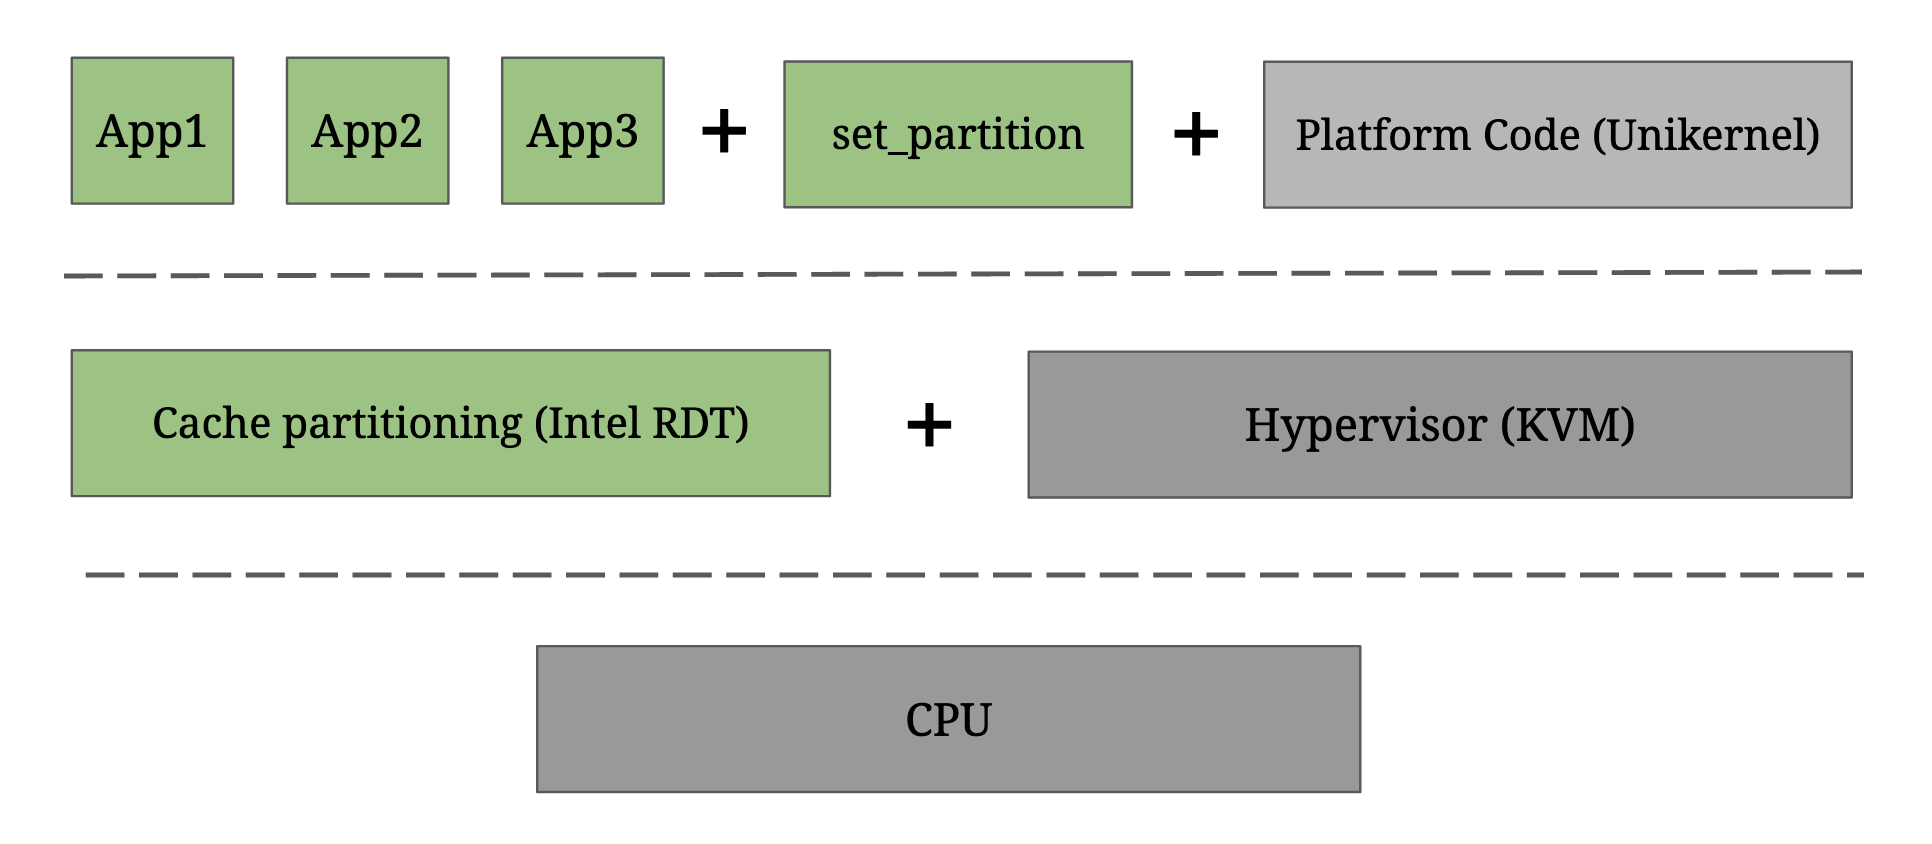
\includegraphics[width=\linewidth]{solution_architecture}
    \label{fig:solution}
    \vspace{-2em}
    \caption{Solution architecture}
    \Description{Brief representation of our contributions at different layers.
    Boxes in green represent our contribution and boxes in grey are the existing
    systems that are being reused}
\end{figure}

We provide an overview of our solution architecture in Fig.2. The boxes in green
represent our own contribution and the grey boxes represent the existing
components that we have reused. We start with the description of the
$\texttt{set\_partition}$ application programming interface (API). The
application has access to an intrinsic function called
$\texttt{set\_partition(int partition\_id)}$. This allows it to denote an
abstract partition for each section of the program. We expect the programmer to
instrument their applications with calls to this function using different
partition IDs to denote which section the program is executing in. For example,
a programmer may denote the networking parts of their application to execute in
partition 1 and computational parts of their application execute in partition 2.
Since these identifiers are abstract, the application can decide the scheme it
uses to partition the application. A simple partitioning scheme would be to
demarcate all network IO into a certain partition and the rest of the
application into another. Further refinements could even create partitions
within the networked section for more fine-grained control. Internally, this
intrinsic function is implemented as a hypercall in the hypervisor. A hypercall
is a mechanism for the user program to signal to the hypervisor that it needs
access to a special resource. This hands over control to the hypervisor which
performs the necessary operations to hand over control of the resource and
returns to the user program. Next, we describe the unikernel library - Unikraft,
that we use to turn our programs into unikernels. A unikernel library is a
specialized library that provides the necessary platform code to turn an
application in a bare-metal kernel. This kernel can now directly execute
on hardware (though it requires a hypervisor to provide some basic platform
abstractions). The advantage of this approach is that only the necessary code
needed to run the application is pulled into the final application binary.
Code for unnecessary features such as virtual memory, scheduling, IO emulation
and others is not present in the kernel and so the memory footprint of these
features is avoided. Unikraft \cite{unikraft} is a library OS, that provides the
necessary platform code and a build system to turn regular applications into
unikernels. These unikernels can be executed on a variety of hypervisors such as
KVM and Xen. It has implementations of standard POSIX compatible system calls
and external libraries can be ported to the Unikraft environment for additional
features. All the applications that we wrote for performance evaluation were
turned into unikernels using Unikraft and then executed on a hypervisor. We also
had to port additional libraries to support our applications. Next, we provide
details of the KVM hypervisor and how we integrated our cache partitioning
scheme into the hypervisor. There are two types of hypervisors, Type-I and
Type-II hypervisors. Type-I hypervisors run directly on the CPU and provide
isolation and platform abstraction features. Type-II hypervisors are intergrated
with an existing operating system and reuse the features of the operating
system to provide platform abstraction. Both types of hypervisors use hardware
virtualization to provide isolation and fast emulation of platform features. In
our setup, we have used the KVM hypervisor, which is integrated with the Linux
operating system and uses Intel VT-d to provide hardware virtualization. KVM has
support for intercepting hypercalls from guest kernels that it is running. It is
in this subsystem that we implement our cache-partitioning feature. We implement
a new hypercall which intercepts calls to $\texttt{set\_partition}$ from the
guest OS. Then, we inspect the partition ID provided by the guest OS and use it
to allot it to a cache partition. An important nuance to keep in mind is that
the guest OS may be executing on a different hardware thread than where the
hypervisor intercepted it. Thus it is important to use the features of KVM to
signal the correct core to allot the cache partition. Further, the choice of
allocation policy also plays an important role in the effectiveness of the
solution. Here we implement a simple round-robin scheme which allocates each new
call to a different partition.

\begin{figure}[h]
  \centering
  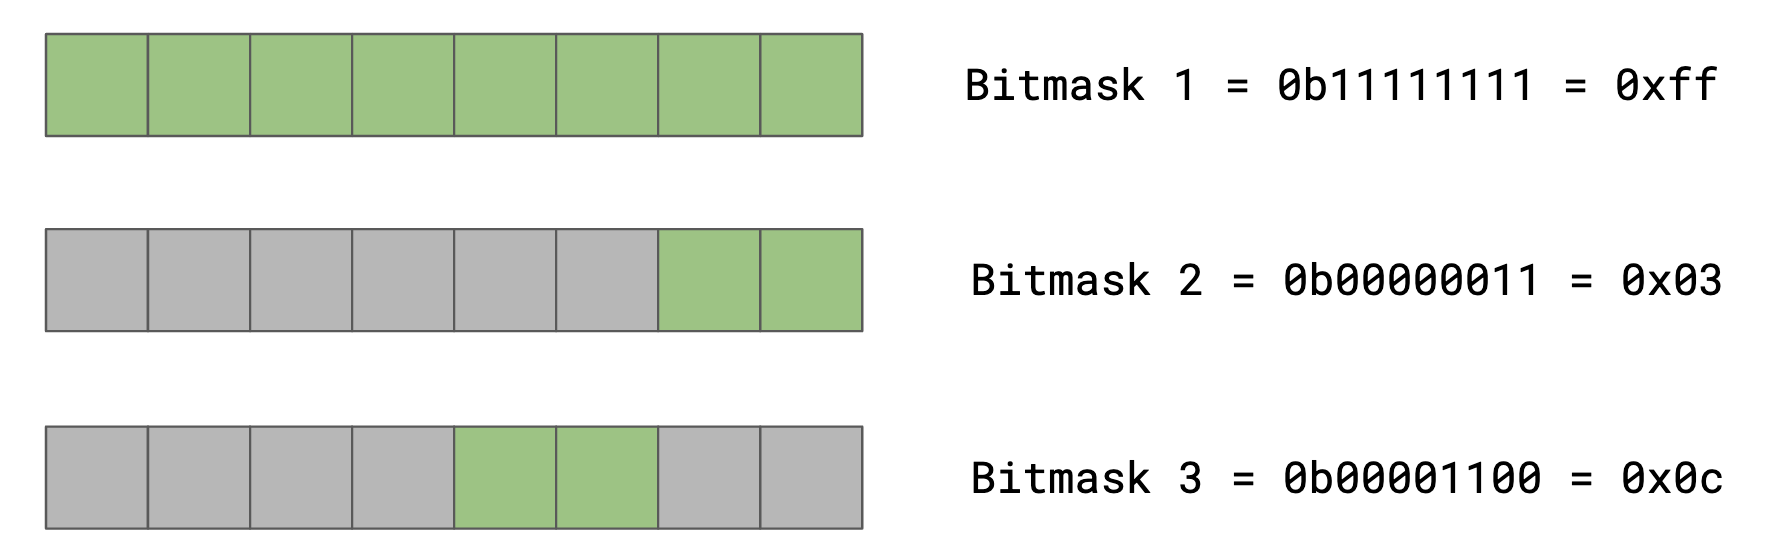
\includegraphics[width=\linewidth]{bitmasks}
    \label{fig:bitmasks}
    \vspace{-2em}
    \caption{Example of cache bitmasks}
\end{figure}

Finally, this allotment is performed using the Intel Resource Director
Technology (RDT). Intel RDT has a subfeature called Cache Allocation Technology
(CAT) which is a hardware feature that allows application level cache
partitioning. The first key component of CAT is the cache bitmask. A cache
bitmask is a fixed size bitstring that is used to represent the regions of the
cache that the application may occupy. We show some examples of bitmasks in
Figure 3. As can be seen, a 1 represents a cache region that an application may
occupy whereas a 0 represents a region it cannot. Thus, Bitmask 1 represents
access to the full cache and Bitmasks 2 and 3 to smaller sections of it. Notice
that Bitmask 2 and 3 are non-overlapping, thus applications execute under these
bitmasks will not interfere with the cache footprint of each other. Each
processor supports a fixed number of bitmasks to be preprogrammed in the system.
Once this is done, we can write a model-specific register in each logical core
which denotes which bitmask the current application should run under. This has
the effect of partitioning the cache such that the requests from the core now go
to the specific cache partition. We use this feature to dynamically switch cache
partitions whenever an application requests a $\texttt{set\_partition}$ call.

\section{Evaluation and Results}

The evaluation of our implementation requires careful analysis because there are
two competing effects at play. On one hand, partitioning cache space for the
networking parts may improve the effectiveness of DDIO by preventing the
eviction of RX/TX buffers. But on the other hand, this may reduce the cache
space available for the remaining parts of the application. Thus, even though
the performance of the networking parts improves the overall application
performance may suffer. Moreover, since our dynamic cache partitioning scheme is
implemented using hypercalls in an hypervisor, there is an overhead associated
with the VM exit. If these events are too frequent, it may add a non-negligible
overhead leading to an increase in runtime. Given this, it would not be possible
to determine the impact of our work by simply measuring wall-clock time. While
an improvement in wall-clock time is beneficial, it does not provide any insight
into which part of our solution resulted in this improvement. In the case that
performance is reduced, we need a method of diagnosing what led to the decrease
in performance. To deal with this, we use statistical profiling of hardware
performance counter events to benchmark different aspects of an application. We
briefly hardware counter events and how they are recorded to better understand
how we use it in our evaluation method. Modern processors have hardware
counters, that count the number of occurences of certain hardware events. These
counters can capture counts ranging from CPU events such as instructions
executed, cycles spent stalling and others, all the way upto system events such
as memory requests, cache hits and misses and so on. Since constantly reading
these counters will have a very high overhead, the processor can be programmed
to generate an interrupt when a certain count is reached. Thus, this is referred
to as statistical profiling, since we only capture a subset of the events. But
the relative values of these counts can give us a good idea if the frequency of
a certain event increased or decreased. Thus we use statistical profiling,
through tools like $\texttt{perf}$ to capture the frequency of certain events
that we believe helps us understand the behavior of our application. First, we
focus on PCIE Writes / Reads from the last level cache (LLC). This is the
primary event that identifies if our solution is working. This event provides
information about the number of PCIE accesses that were serviced from the LLC.
This is important because if we are servicing more requests from the LLC, this
implies that more network packets are staying resident in the cache and directly
being processed from there, instead of being retrieved from main memory. Second,
we focus on the total LLC Misses in the application. This is important because
by partitioning the cache there is a chance we increase the number of cache
misses in the application. Thus, we would like to analyze if the total number of
application cache misses is increasing substantially. Finally, we also measure
application level benchmarks such as bandwidth and latency of requests served,
since finally any improvement in the software should result in an observed
improvement in the client side performance. We have implemented four benchmarks
- (1) \textbf{CS}: This program implements the Websocket protocol over TCP and
creates a chat server. (2) \textbf{ML}: This program implements different ML
algorithms to perform packet based quality-of-service classification (3)
\textbf{KV} : This program implements a replicated key-value store using
leader-server replication (4) \textbf{DL} : This program implements a deep
learning inference workload for image recognition We believe this set of
benchmarks are representative because they capture different types of workloads.
\textbf{CS} is mostly network IO with little computation since it only performs
Websocket packet-framing and forwarding over TCP. \textbf{ML} and \textbf{DL}
represent a balance between network IO and compute, since the inference
procedure requires non-trivial amounts of computation. Finally, \textbf{KV}
represents a combination of network IO and disk IO, since the records are stored
on the filesystem. Thus, evaluating the performance of our solution over these
benchmarks should help us understand how it works. All of our benchmarks are
executed on an AWS m5zn.metal machine with 48 logical cores, running on Amazon
Linux 2, using QEMU 6.0.0 and Unikraft 0.10.0. We have 4 test scenarios - (1)
\textbf{OS} : run the application on the OS, (2) \textbf{OS+PT} : run the
application on the OS stack + fine-grained partitioning, (3) \textbf{UK} : run
the application as a unikernel, (4) \textbf{UK+PT} : run the application as a
unikernel + fine-grained partitioning. This will help to evaluate the effect of
each component of our solution. In the following figures, we present and discuss
our results. Note that the absolute numbers of the hardware counters are
normalized, to make comparison easier. 

First, we observe the PCIe hits for each benchmark in Fig.4. Across all setups,
we note that the PCIe hits increases. In the case of \textbf{OS+PT} case, this
is not significant, implpying that the OS interference is removing any benefits
that we may observe. In the \textbf{UK} and \textbf{UK+PT} case, we observe that
the PCIe hits increases. This shows that our cache partitioning has the effect
of isolating network buffers, so that PCIe hits are increased. The rate of
increase across different applications is different because of various network
packet parameters such as size of packets, number of packets received and so on.

\begin{figure}[h]
  \centering
  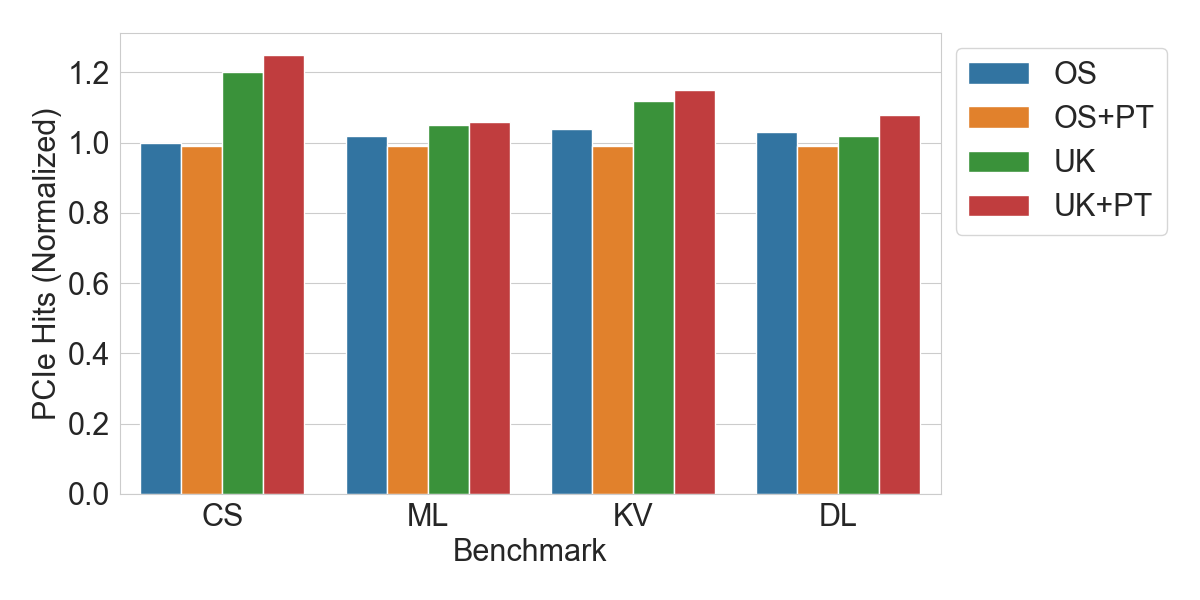
\includegraphics[width=\linewidth]{res1}
    \label{fig:motivating}
    \vspace{-2em}
    \caption{PCIe Hits for each benchmark}
\end{figure}

Next we move to the LLC misses observed for each benchmark. As shown in Fig. 5.,
LLC misses drop consistently when we move from \textbf{OS} to \textbf{UK}. This
is because the smaller memory footprint of the unikernel allows more cache space
for the application, thus reducing the number of cache misses. But, our
partitioning scheme increases the cache misses, whether it is added to
\textbf{OS} or \textbf{UK}. This is expected, since the computational parts of
the application are receiving less cache space, more cache misses are expected.
In the case of the compute heavy benchmarks such as \textbf{ML} and \textbf{DL},
we observe that cache misses are significantly increased, since they perform lot
of computation. In the case of \textbf{KV} and \textbf{ML}, this is less since
they are not peforming too much computation and are mostly IO bound.

\begin{figure}[h]
  \centering
  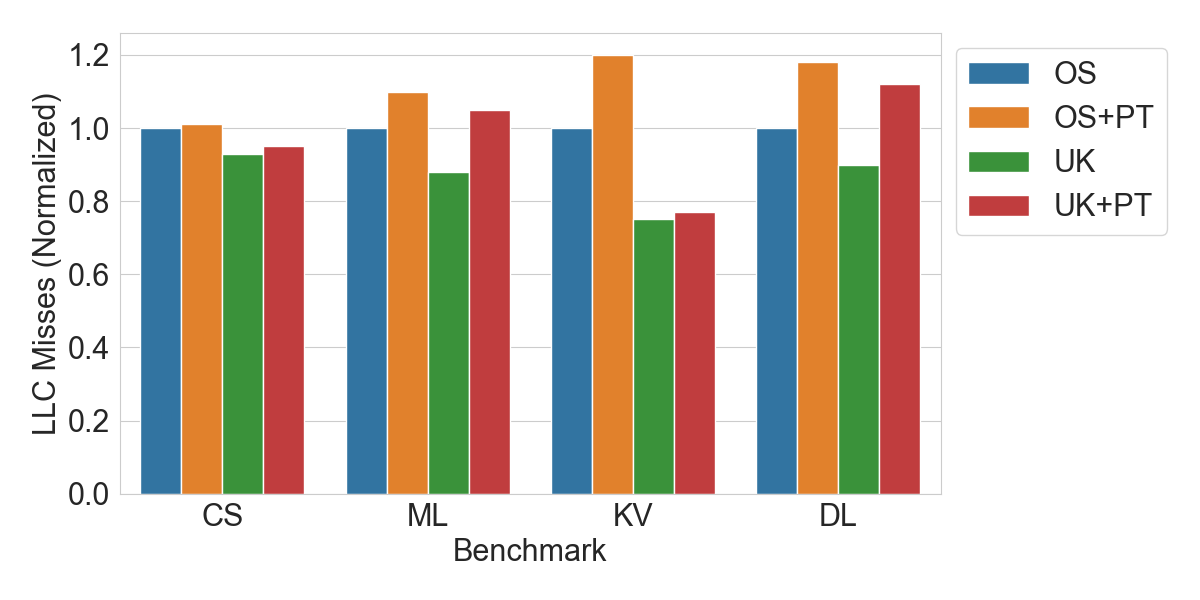
\includegraphics[width=\linewidth]{res2}
    \label{fig:motivating}
    \vspace{-2em}
    \caption{LLC Misses for each benchmark}
\end{figure}

In Fig. 6, we discuss the results of our throughput experiments. For each
application, we setup multiple clients who then send requests to saturate the
link and we check how many requests per second we can serve. We note that
throughput increases for most benchmarks when going from \textbf{OS} to
\textbf{UK} due to the smaller memory footprint and less cache contention. In
the case of the \textbf{CS} and \textbf{KV} benchmarks we see an increase in the
performance due to our partitioning scheme. But in the case of \textbf{DL} and
\textbf{ML}, there is a drop in the performance. Our hypothesis is that since
\textbf{CS}, \textbf{KV} are IO dominated, our scheme isolates the network
buffer and improves the networking performance which translates to an
improvement in the overall application performance. obtained. In the \textbf{DL}
and \textbf{ML} case, it is possible that the smaller cache allocation is
increasing the time taken to perform the computationally heavy part so much that
any improvements in the networking part are mitigated. This is reasonable,
since these programs are very sensitive to the cache size.

\begin{figure}[h]
  \centering
  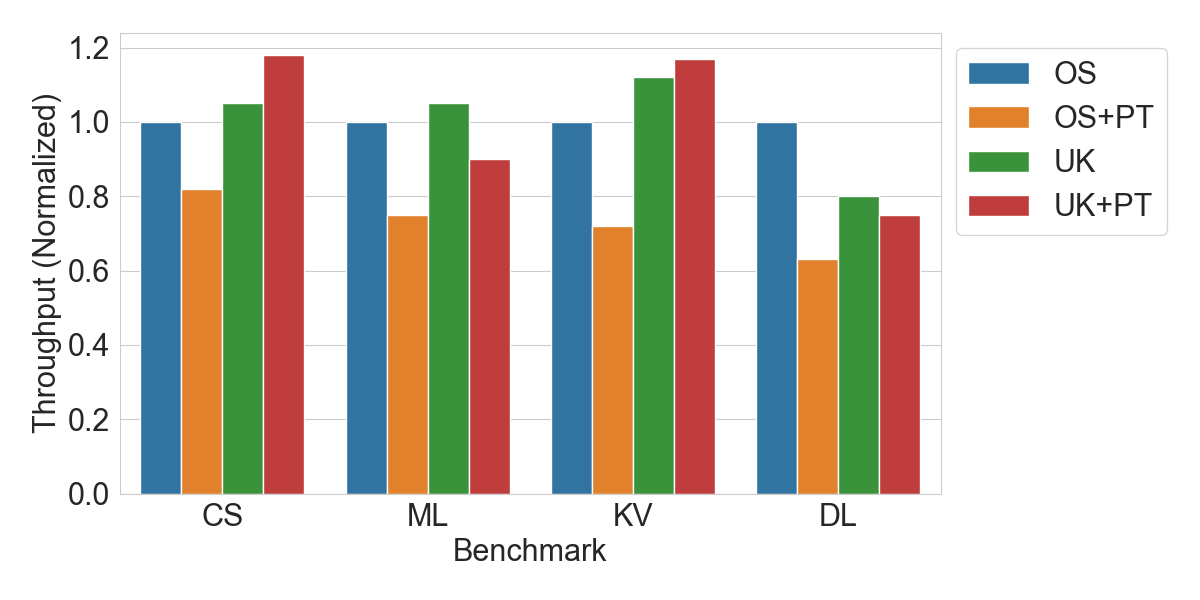
\includegraphics[width=\linewidth]{res3}
    \label{fig:motivating}
    \vspace{-2em}
    \caption{Throughput for each benchmark}
\end{figure}

Finally, we observe the P99 latency for the various benchmarks in Fig. 7. As
observed, the P99 latency improves (smaller is better) for only the \textbf{CS}
benchmark and gets worse for all others. A similar hypothesis from the
throughput section applies, where any improvement in the networking parts of the
code are mitigated by the rest of the application. Moreover, limiting the cache
space may have the unforeseen effect of evicting some packets, which were
previously able to be served from the cache, thus increasing the P99 latency.

\begin{figure}[h]
  \centering
  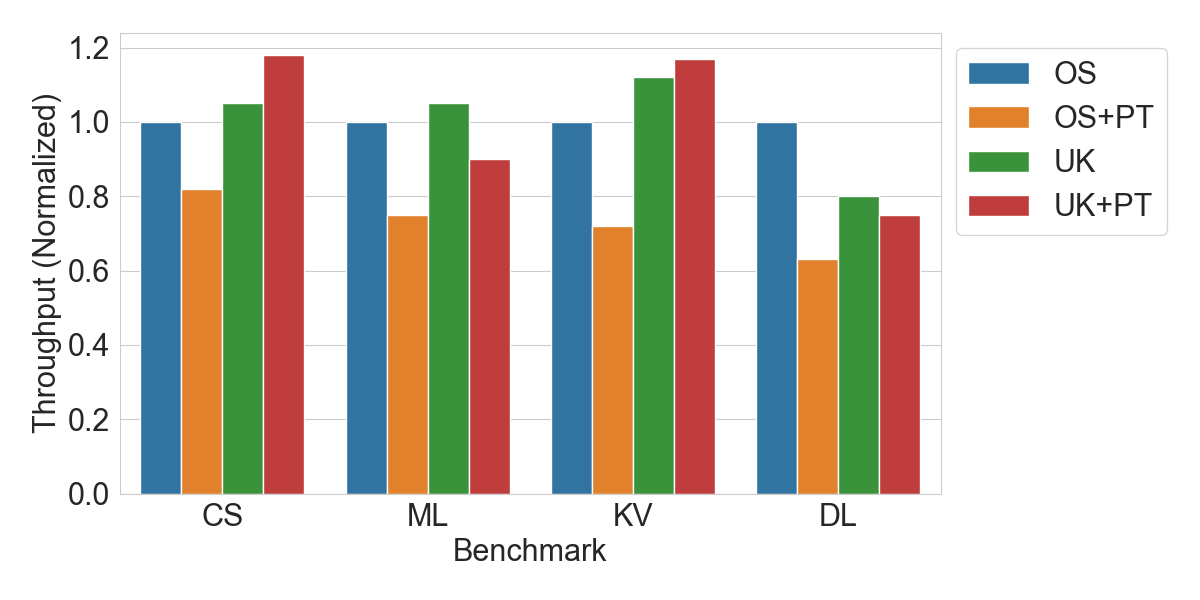
\includegraphics[width=\linewidth]{res3}
    \label{fig:motivating}
    \vspace{-2em}
    \caption{P99 Latency for each benchmark}
\end{figure}

\section{Related Work}
The work most closely related to our work is \cite{alireza_2020}. The work
performs a thorough analysis of the Intel DDIO implementation. Their experiments
consider different types of applications executed under different cache
partitioning schemes. The major takeaway from their work that we capitalized on
was that there is no \textit{one-size-fits-all} cache partitioning policy. Thus
we implement a solution that allows an application to customize its use of the
cache, tailored to its specific needs. On the front of fine-grained
cache-partioning, there are two main directions - software based cache
partitioning based on colored pages \cite{herter}, \cite{sherwood} and hardware
based way partitioning (such as Intel RDT) \cite{chen}, \cite{assaf}. The work
closest to our implementation is \cite{swap}, which also proposes a fine-grained
cache partitioning scheme. But their work does not consider the effect of this
scheme on networked applications. Further the implementation is not performed
using Intel RDT (which is a more mainstream implementation of hardware cache
partitioning) and also does not take into the effect of hypervisor (necessary
for safe isolation of applications).

\section{Conclusion and Future Work}

We have designed and implemented a solution to reduce the effect of cache
contention on the performance of network IO and demonstarted our results. While
the results are not promising, since we do not see a consistent improvement in
performance across all the benchmarks, the \textbf{CS} and \textbf{KV}
benchmarks provide insight into situations where this solution may work.
Additionally, it also corroborates the claim of \cite{alireza_2020} that heavily
CPU or memory bound applications do not benefit much from DDIO tuning based on
cache partitioning as observed in \textbf{ML} and \textbf{DL}. Still, I feel
this work opens up interesting future directions. The first and most important
learning is that this technique can be specialized for specific applications
such as virtual switches, network function virtualization and similar
applications which are dominated by network IO. Further, the cache allocation
policy needs a thorough review to ensure that it is performing optimally. This
would require digging deeper into the cache allocation being performed by our
simple round-robin algorithm and how it can be improved. On the measurement
front, we feel there are multiple things that can be improved to make this work
better. First, the network stack used in the \textbf{OS} and \textbf{UK} setup
is different, since we could only port a simple TCP/IP stack to the unikernel
environment. It would be good to have something like DPDK tuned for both the
setups, thus giving a better comparison. If a fair baseline is established
between the OS and unikernel setup, then we can be confident that our
implementation improves the performance of the application. Second, the
measurements are performed in noisy environments, because the Linux kernel is
still running on the cores that are running the unikernels. Isolating these
cores requires the use of advanced features such as ISOLCPUs, which are not
available in the EC2 instances that we used. Thus, we believe that we have made
a case for intra-application cache partitioning and unikernels.

\begin{acks}
    To Prof. Muhammad Shahbaz for conducting such a great course and Sharuna
    Anandraj, Darwin Kamanuru, K M A Solaiman and Kai Ling for helping out
    throughout the semester!
\end{acks}

%%
%% The next two lines define the bibliography style to be used, and
%% the bibliography file.
\bibliographystyle{ACM-Reference-Format}
\bibliography{db}


%%
%% If your work has an appendix, this is the place to put it.
\appendix

\section{Contributions}

\subsection{Jiangqiong Liu}
Worked on the handling the measurement across the entire project. Implemented
perf scripts to automate collection of hardware counter events for all
applications and perform the post-processing to report the results. Correlated
performance changes in application based on measurement results.

\subsection{Joshua Reprogle}
Implemented an end-to-end Websocket server in C++ and used it to implement a
chat server. The C++ server was written without dynamic memory allocation to
carefully control the placement of memory buffers. Identified networking parts
of the application and performed $\texttt{set\_partition}$ instrumentation.

\subsection{Vedaant Rajoo}
Implemented a replicated, in-memory key-value store using C++. Analyzed
networking and computational parts of the application and performed
$\texttt{set\_partition}$ instrumentation.

\subsection{Sowmya Jayaram Iyer}
Implemented machine learning models for packet based classification. Executed
these models on real-world traces and ported them to run as Unikraft kernels.
Identified the $\texttt{set\_partition}$ instrumentation points for compute
bound parts of the application.

\subsection{Keerthana Ashokkumar}
Designed and implemented a replicated, in-memory key-value store using Java.
Implemented two phase commit based atomic updates and leader server replication.
Assisted in the C++ implementation of the in-memory store and identified
networking parts of the application.

\subsection{Anmol Sahoo}
Designed and implemented the Intel RDT based cache partitioning scheme as a KVM
patch in the Linux kernel. Exposed the userspace API as VMCALLs in KVM. Ported
the necessary libraries to Unikraft (rpclib for rpc, tcp/ip for sockets, tvm for
deep learning / machine learning). Performed end-to-end execution and testing of
all applications.

\end{document}

\endinput
%%
%% End of file `sample-sigconf.tex'.
